\documentclass[aspectratio=169,13pt,t] {beamer}
%
% Choose how your presentation looks.
%
% For more themes, color themes and font themes, see:
% http://deic.uab.es/~iblanes/beamer_gallery/index_by_theme.html
%
\mode<presentation>
{
  \usetheme{Madrid}      % or try Darmstadt, Madrid, Warsaw, ...
  \usecolortheme{beaver} % or try albatross, beaver, crane, ...
  \usefonttheme{serif}  % or try serif, structurebold, ...
  \setbeamertemplate{navigation symbols}{
  	\insertslidenavigationsymbol
  	\insertdocnavigationsymbol}
  \setbeamertemplate{caption}[numbered]
  \setbeamertemplate{items}[default]
}

\usepackage[,UTF8,linespread=1.2]{ctex}
\usepackage{wrapfig}
\usepackage{caption}
\captionsetup[figure]{name=图,labelsep=period}
\usepackage[,most]{tcolorbox}
\usepackage{picinpar}
\usetikzlibrary{intersections,calc}

\usepackage{xcolor}
\definecolor{xy_blue}{cmyk}{0.6,0.35,0.0,0.4}
\definecolor{xy_orange}{cmyk}{0.0,0.7,1.0,0.0}
\definecolor{xy_green}{cmyk}{0.2,0.0,1.0,0.15}
\xdefinecolor{xy_gold}{RGB}{135,103,79}
\xdefinecolor{xy2_gold}{cmyk}{0,0.35,0.75,0.05}
% 自定义颜色
\definecolor{myblue}{RGB}{0, 112, 192}
\definecolor{myorange}{RGB}{237, 125, 49}
\definecolor{mygreen}{RGB}{0, 176, 80}

\setbeamercolor{section number projected}{fg=red,bg=red!20}%控制球的颜色
\setbeamercolor{subsection number projected}{fg=blue,bg=blue!40}
\setbeamercolor{item}{fg=xy_gold} %设置列表项颜色

\usepackage{amsthm}
\newtheorem{peroration}{结论：}
\newtheorem{exploration}{探究：}
\newtheorem*{prooft}{证明：}
\newtheorem{question}{问题}
\newtheorem*{solve}{解:}
\newtheorem{instance}{例}   % 解：独立计数器
\BeforeBeginEnvironment{peroration}{%
	\setbeamercolor{block title}{bg=xy_green,fg=white}
	\setbeamercolor{block body}{bg=xy_green!10}
}
\AfterEndEnvironment{peroration}{
	\setbeamercolor{block title}{bg=xy_blue,fg=white}
	\setbeamercolor{block body}{bg=xy_blue!10}
}
\BeforeBeginEnvironment{exploration}{%
	\setbeamercolor{block title}{bg=xy_orange,fg=white}
	\setbeamercolor{block body}{bg=xy_orange!10}
}
\AfterEndEnvironment{peroration}{
	\setbeamercolor{block title}{bg=xy_blue,fg=white}
	\setbeamercolor{block body}{bg=xy_blue!10}
}
\BeforeBeginEnvironment{solution}{%
	\setbeamercolor{block title}{bg=xy_green,fg=white}
	\setbeamercolor{block body}{bg=xy_green!10}
}
\AfterEndEnvironment{solution}{
	\setbeamercolor{block title}{bg=xy_green,fg=white}
	\setbeamercolor{block body}{bg=xy_green!10}
}
\BeforeBeginEnvironment{prooft}{%
	\setbeamercolor{block title}{bg=xy_green,fg=white}
	\setbeamercolor{block body}{bg=xy_green!10}
}
\AfterEndEnvironment{prooft}{
	\setbeamercolor{block title}{bg=xy_green,fg=white}
	\setbeamercolor{block body}{bg=xy_green!10}
}
\BeforeBeginEnvironment{question}{%
	\setbeamercolor{block title}{bg=xy_orange,fg=white}
	\setbeamercolor{block body}{bg=xy_orange!10}
}
\AfterEndEnvironment{question}{
	\setbeamercolor{block title}{bg=xy_green,fg=white}
	\setbeamercolor{block body}{bg=xy_green!10}
}
\BeforeBeginEnvironment{solve}{%解：
	\begingroup
	\setbeamercolor{block title}{bg=xy_orange!60,fg=white}
	\setbeamercolor{block body}{bg=xy_orange!10}
}
\AfterEndEnvironment{solve}{%解：
	\endgroup
}

\setbeamercolor{prooft}{fg=red, bg=green!10}       % 标题颜色
\setbeamercolor{prooft body}{fg=red, bg=red!5}  % 内容块背景
\setbeamerfont{prooft head}{series=\bfseries}       % 标题字体
\setbeamerfont{question body}{shape=\upshape}         % 内容字体
\renewcommand{\thefigure}{\arabic{figure}}

\newtcolorbox{summarybox}[1][]{
	colback=purple!10,
	colframe=purple!70!black,
	fonttitle=\bfseries,
	title=#1,
	arc=1mm,
	boxrule=0pt,drop shadow,
	left=2mm, right=2mm, top=2mm, bottom=2mm,
}
\newtcolorbox{summarybox-answer}{
%	width=0.9\textwidth,
	colback=white,
	blanker,
	borderline west={2pt}{2pt}{cyan},
	left=2mm, right=2mm, top=2mm, bottom=2mm,
	}
\title[3.2.1 单调性与最大(小)值]{3.2.1 单调性与最大(小)值}
\subtitle{增函数与减函数、单调区间}
\author[好好学习，努力向上]{}
\institute{}
\date{2026.10.19}
%\setbeamertemplate{theorems}[numbered]
\theoremstyle{definition}
\newtheorem{exam}{例}
\AtBeginSection[]
{
  \begin{frame}<beamer>
    \frametitle{本节主要内容}
    \tableofcontents[currentsection,currentsubsection]
  \end{frame}
}

\AtBeginDocument{
	\setlength{\abovedisplayskip}{3pt}
	\setlength{\belowdisplayskip}{3pt}
	\setbeamertemplate{theorems}[numbered]
}

\usepackage{pgfplots}
\pgfplotsset{compat=1.18}
\usetikzlibrary{arrows.meta}

\begin{document}
\begin{frame}{}
	\titlepage
\end{frame}

\begin{frame}{内容概览}
	\tableofcontents
\end{frame}

\section{单调性的概念}

\begin{frame}{观察：二次函数 \(f(x)=x^2\) 的图象}
	在初中，我们利用函数图象研究过函数值随自变量增大而增大（或减小）的性质，这一性质叫做函数的\textbf{单调性}.
	\begin{columns}[t]
		\column{0.40\textwidth}\hspace{2em}
		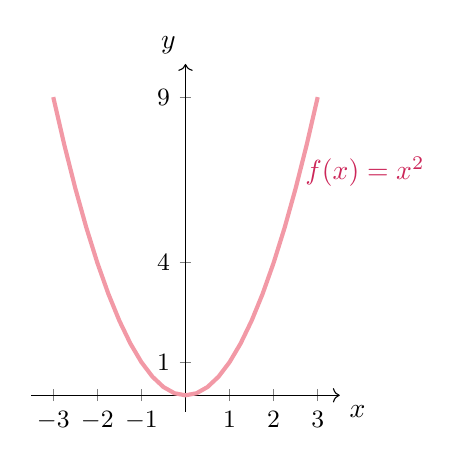
\begin{tikzpicture}[baseline=3cm]
			\begin{axis}[
				clip=false,
				width=5.5cm, height=6cm,
				xmin=-3.5, xmax=3.5,
				ymin=-0.5, ymax=10,
				xtick={-3,-2,-1,0,1,2,3},
				ytick={1,4,9},
				axis lines=middle,
				axis line style={->},
				xlabel={$x$}, ylabel={$y$},
				xlabel style={below right},
				ylabel style={above left},
				tick label style={font=\small},
			]
			\addplot[color=pink!80!purple, line width=1.5pt, domain=-3:3] {x^2};
			\node[above right, pink!20!purple] at (2.5, 6) {$f(x)=x^2$};
			\end{axis}
		\end{tikzpicture}

	
		\column{0.6\textwidth}
		\begin{minipage}{\textwidth}
		\begin{summarybox-answer}
			图象在 \(y\) 轴左侧从左到右\textbf{下降}：当 \(x\leqslant 0\) 时，\(y\) 随 \(x\) 增大而减小.\\[4pt]
			图象在 \(y\) 轴右侧从左到右\textbf{上升}：当 \(x\geqslant 0\) 时，\(y\) 随 \(x\) 增大而增大.
		\end{summarybox-answer}
	\end{minipage}
	\end{columns}
\end{frame}

\begin{frame}{增函数与减函数的定义}
	\pause
	一般地，设函数 \(f(x)\) 的定义域为 \(D\)，区间 \(I\subseteq D\)：
	\pause
	\begin{summarybox}[单调递增]
	如果 \(\forall x_1,x_2\in I\)，当 \(x_1<x_2\) 时，都有 \(f(x_1)<f(x_2)\)，那么称函数 \(f(x)\) 在区间 \(I\) 上\textbf{单调递增}.
	\end{summarybox}
	\pause
	\begin{summarybox}[单调递减]
	如果 \(\forall x_1,x_2\in I\)，当 \(x_1<x_2\) 时，都有 \(f(x_1)>f(x_2)\)，那么称函数 \(f(x)\) 在区间 \(I\) 上\textbf{单调递减}.
	\end{summarybox}
	\vspace{0.5em}
	\pause
	\begin{summarybox-answer}
	特别地，当函数在它的定义域上单调递增时，称它是\textbf{增函数}；单调递减时，称它是\textbf{减函数}. 区间 \(I\) 叫做函数的\textbf{单调区间}.
	\end{summarybox-answer}
\end{frame}

\begin{frame}{图象直观：上升与下降}
	\begin{columns}
		\column{0.5\textwidth}
		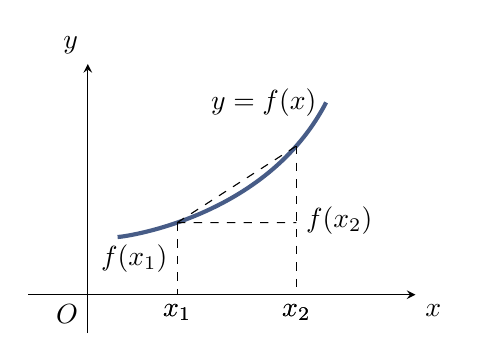
\begin{tikzpicture}[baseline={(0,0)}]
			\begin{axis}[
				clip=false,
				width=6.5cm, height=5cm,
				xmin=-1, xmax=5.5, ymin=-1, ymax=6,
				xtick=\empty, ytick=\empty,
				axis lines=middle, axis line style={->},
				xlabel={$x$}, ylabel={$y$},
				xlabel style={below right}, ylabel style={above left},
				>=stealth,
			]
			\draw[name path =curve,line width=1.5pt,color=xy_blue] 
				(0.5,1.5) .. controls (0.6,1.5) and (3.0,2) .. (4,5);
			\path [name path =a_1] (1.5,0) -- (1.5,5);
			\path [name path = b_1] (3.5,0) -- (3.5,5);
			\path [name intersections={of =curve and a_1,by=a}]  ;
			\path [name intersections={of =curve and b_1,by=b}]  ;
			\draw[dashed] (a) -- (a |- 0,0)node[below]{$x_1$};
			\draw[dashed] (b) -- (b |- 0,0)node[below]{$x_2$};
			\draw [dashed] (a) -|(a -| b) (a) -- (b);
			\node[below] at (1.5,0) {$x_1$};
			\node[below] at (3.5,0) {$x_2$};
			\node[left] at ($(a)!0.5!(a |- 0,0)$) {$f(x_1)$};
			\node[right] at ($(b)!0.5!(b |- 0,0)$) {$f(x_2)$};
			\node[left] at (4,5) {$y=f(x)$};
			\node[below left] at (0,0) {$O$};
			\end{axis}
		\end{tikzpicture}
		
		\centering\small 单调递增（上升）
		\captionof{figure}{}
		
		\column{0.5\textwidth}
		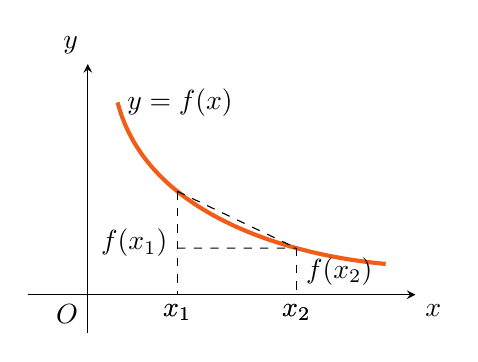
\begin{tikzpicture}[baseline={(0,0)}]
			\begin{axis}[
				clip=false,
				width=6.5cm, height=5cm,
				xmin=-1, xmax=5.5, ymin=-1, ymax=6,
				xtick=\empty, ytick=\empty,
				axis lines=middle, axis line style={->},
				xlabel={$x$}, ylabel={$y$},
				xlabel style={below right},
				ylabel style={above left},
				>=stealth,
			]
			\draw[name path=curve,line width=1.5pt,color=xy_orange] (0.5,5) .. controls (1,2) and (3.5,1) .. (5,0.8);
			\path [name path =a_1] (1.5,0) -- (1.5,5);
			\path [name path = b_1] (3.5,0) -- (3.5,5);
			\path [name intersections={of =curve and a_1,by=a}]  ;
			\path [name intersections={of =curve and b_1,by=b}]  ;
			\draw[dashed] (a) -- (a |- 0,0)node[below]{$x_1$};
			\draw[dashed] (b) -- (b |- 0,0)node[below]{$x_2$};
			\draw [dashed] (a |- b) -- (b) (a) -- (b);
			\node[below] at (1.5,0) {$x_1$};
			\node[below] at (3.5,0) {$x_2$};
			\node[left] at ($(a)!0.5!(a |- 0,0)$) {$f(x_1)$};
			\node[right] at ($(b)!0.5!(b |- 0,0)$) {$f(x_2)$};
			\node[right] at (0.5,5) {$y=f(x)$};
			\node[below left] at (0,0) {$O$};
			\end{axis}
		\end{tikzpicture}
	
		\centering\small 单调递减（下降）	
		\captionof{figure}{}
	\end{columns}
\end{frame}

\section{单调性的证明}

\begin{frame}{例1：研究 \(f(x)=kx+b\,(k\neq 0)\) 的单调性}
	
	\pause\vspace{-1em}
	\begin{solve}
	\pause
	函数 \(f(x)=kx+b\) 的定义域是 \(\mathbf{R}\). 任取 \(x_1,x_2\in\mathbf{R}\)，且 \(x_1<x_2\)，则
	\[
		f(x_1)-f(x_2)=(kx_1+b)-(kx_2+b)=k(x_1-x_2).
	\]
	由 \(x_1<x_2\)，得 \(x_1-x_2<0\).
	\begin{enumerate}[(1)]
	\item<4-> 当 \(k>0\) 时，\(k(x_1-x_2)<0\)，于是 \(f(x_1)-f(x_2)<0\)，即 \(f(x_1)<f(x_2)\).\\
	\quad 这时 \(f(x)=kx+b\) 是\textbf{增函数}.
	\item<5-> 当 \(k<0\) 时，\(k(x_1-x_2)>0\)，于是 \(f(x_1)-f(x_2)>0\)，即 \(f(x_1)>f(x_2)\).\\
	\quad 这时 \(f(x)=kx+b\) 是\textbf{减函数}.
	\end{enumerate}
	\end{solve}
	
	\pause\pause\pause
	\begin{summarybox-answer}
		\textbf{证明四步}：取值（设 \(x_1<x_2\)）\(\to\) 作差 \(f(x_1)-f(x_2)\)\(\to\) 变形（因式分解）\(\to\) 定号（判断与 \(0\) 的大小）.
	\end{summarybox-answer}
\end{frame}

\begin{frame}{例2. 物理学中的玻意耳定律 \(p=\frac{k}{V}\)（\(k\) 为正常数）告诉我们，对于一定量的气体，当其体积 \(V\) 减小时，压强 \(p\) 将增大. 试对此用函数的单调性证明.}
	
\vspace{-2em}
	\begin{prooft}
	\pause
	 \(\forall V_1, V_2 \in (0, +\infty)\)，且 \(V_1 < V_2\)，则
	\[
	p_1 - p_2 = \frac{k}{V_1} - \frac{k}{V_2} = k\frac{V_2 - V_1}{V_1V_2}.
	\]
	\pause
	由 \(V_1, V_2 \in (0, +\infty)\)，得 \(V_1V_2 > 0\)；
	由 \(V_1 < V_2\)，得 \(V_2 - V_1 > 0\).
	又 \(k > 0\)，于是
	\[
	p_1 - p_2 > 0,
	\]
	即
	$p_1 > p_2.$
	
	\pause
	所以，根据函数单调性的定义，函数 \(p=\frac{k}{V}\)，\(V \in (0, +\infty)\) 是减函数. 也就是说，当体积 \(V\) 减小时，压强 \(p\) 将增大.
\end{prooft}

	\pause\vspace{-1em}
\begin{summarybox-answer}
	\textbf{步骤}：作差 --- 变形 --- 符号.
\end{summarybox-answer}
\end{frame}



\begin{frame}{例3：证明 \(y=x+\dfrac{1}{x}\) 在 \((1,+\infty)\) 上单调递增}
	\pause
	\vspace{-1em}
	\begin{prooft}[]
	任取 \(x_1,x_2\in(1,+\infty)\)，且 \(x_1<x_2\)，有
	\[
		y_1-y_2=\Bigl(x_1+\frac{1}{x_1}\Bigr)-\Bigl(x_2+\frac{1}{x_2}\Bigr)
		=(x_1-x_2)+\frac{x_2-x_1}{x_1x_2}
		=\frac{x_1-x_2}{x_1x_2}(x_1x_2-1).
	\]
	
	\pause
	由 \(x_1,x_2\in(1,+\infty)\)，得 \(x_1>1,\ x_2>1\)，所以 \(x_1x_2>1\)，即 \(x_1x_2-1>0\).\\
	又由 \(x_1<x_2\)，得 \(x_1-x_2<0\). 于是
	\[
	\frac{x_1-x_2}{x_1x_2}(x_1x_2-1)<0,\quad\text{即 } y_1<y_2.
	\]
	\pause
	所以，函数 \(y=x+\dfrac{1}{x}\) 在区间 \((1,+\infty)\) 上\textbf{单调递增}.
	\end{prooft}
	
	\pause
	\begin{summarybox-answer}
		\textbf{关键}：作差后通过通分、因式分解，把差化成几个因式乘积的形式，再逐一判断符号.
	\end{summarybox-answer}
\end{frame}



\begin{frame}{小结}
	单调性概念：
	\begin{enumerate}[(1)]
		\item<2-> 单调递增
		\item<3-> 单调递减
	\end{enumerate}
\end{frame}

\begin{frame}{布置作业}
	P79 练习 ：1，2，3，4
	
	P85---86 习题3.2： 1，2，4
\end{frame}

	% ---------------------------------------------------------
% 练习 1
% ---------------------------------------------------------
\begin{frame}{练习 1：生产效率与工人数}
	\textbf{\textcolor{myblue}{1.}} 请根据下图描述某装配线的生产效率与生产线上工人数量间的关系.
	
	\begin{columns}
		\begin{column}{0.5\textwidth}
			\begin{tikzpicture}[baseline=( current bounding box.north)]
				\begin{axis}[
					axis lines=middle,
					xlabel={工人数}, ylabel={生产效率},
					xlabel style={below},
					ylabel style={right},
					xmin=-1, xmax=6, ymin=-1, ymax=5,
					xtick=\empty, ytick=\empty,
					width=6cm, height=4.5cm,
					samples=100,
					axis line style={-stealth, thick},
					]
					% (起点) parabola bend (顶点) (终点) 抛物线；
					\draw[magenta,line width=1.5pt] (0,0) parabola bend (2.8,3.5) (5,1.5);
					\node at (axis cs:0,0) [below left] {\(O\)};
				\end{axis}
			\end{tikzpicture}
		\end{column}
		\begin{column}{0.5\textwidth}
			\textbf{解答：}\\
			由图象可知，该函数图象先上升后下降。
			\begin{itemize}
				\item 在生产线上工人数量较少时（图象左侧），随着工人数量的增加，生产效率逐渐提高（单调递增）。
				\item 当工人数量达到一定值后（图象右侧），继续增加工人数量，生产效率反而会降低（单调递减）。
			\end{itemize}
			这说明并不是工人越多越好，存在一个最佳工人数量使生产效率最高。
		\end{column}
	\end{columns}
\end{frame}

% ---------------------------------------------------------
% 练习 2
% ---------------------------------------------------------
\begin{frame}{练习 2：证明一次函数单调性}
	\textbf{\textcolor{myblue}{2.}} 根据定义证明函数 \(f(x)=3x+2\) 是增函数.
	
	\vspace{0cm}
	\textbf{解答：}\\
	函数 \(f(x)=3x+2\) 的定义域为 \(\mathbb{R}\)。
	
	任取 \(x_1, x_2 \in \mathbb{R}\)，且 \(x_1 < x_2\)，则：
	\begin{align*}
		f(x_1) - f(x_2) &= (3x_1 + 2) - (3x_2 + 2) \\
		&= 3x_1 - 3x_2 \\
		&= 3(x_1 - x_2).
	\end{align*}
	因为 \(x_1 < x_2\)，所以 \(x_1 - x_2 < 0\)。
	又因为 \(3 > 0\)，所以 \(3(x_1 - x_2) < 0\)，即：
	\[
	f(x_1) - f(x_2) < 0.
	\]
	从而 \(f(x_1) < f(x_2)\)。
	
	根据函数单调性的定义，函数 \(f(x)=3x+2\) 在 \(\mathbb{R}\) 上是增函数。
\end{frame}

% ---------------------------------------------------------
% 练习 3
% ---------------------------------------------------------
\begin{frame}{练习 3：证明反比例函数单调性}\vspace{-0.5cm}
	\textbf{\textcolor{myblue}{3.}} 证明函数 \(f(x)=-\frac{2}{x}\) 在区间 \((-\infty, 0)\) 上单调递增.
	
	\textbf{解答：}
	任取 \(x_1, x_2 \in (-\infty, 0)\)，且 \(x_1 < x_2\)，则：
	\begin{align*}
		f(x_1) - f(x_2) &= \left(-\frac{2}{x_1}\right) - \left(-\frac{2}{x_2}\right) \\
		&= -\frac{2}{x_1} + \frac{2}{x_2} \\
		&= \frac{-2x_2 + 2x_1}{x_1x_2} \\
		&= \frac{2(x_1 - x_2)}{x_1x_2}.
	\end{align*}
	因为 \(x_1, x_2 \in (-\infty, 0)\)，所以 \(x_1x_2 > 0\)。
	因为 \(x_1 < x_2\)，所以 \(x_1 - x_2 < 0\)。
	因此，\(\frac{2(x_1 - x_2)}{x_1x_2} < 0\)，即 \(f(x_1) - f(x_2) < 0\)。
	所以 \(f(x_1) < f(x_2)\)。
	
	根据函数单调性的定义，函数 \(f(x)=-\frac{2}{x}\) 在区间 \((-\infty, 0)\) 上单调递增。
\end{frame}

% ---------------------------------------------------------
% 练习 4
% ---------------------------------------------------------
\begin{frame}{练习 4：反比例函数的图象与单调性}\vspace{-1em}
	\textbf{\textcolor{myblue}{4.}} 画出反比例函数 \(y=\frac{k}{x}\) 的图象.
	\begin{columns}
		\begin{column}{0.3\textwidth}
			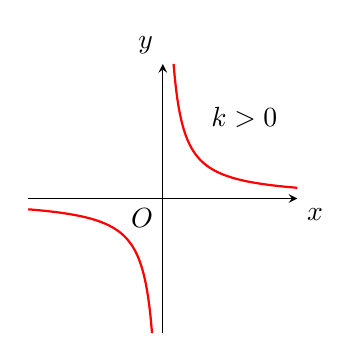
\begin{tikzpicture}[baseline=(current bounding box.north)]
				\begin{axis}[
					axis lines=middle,
					xlabel={\(x\)}, ylabel={\(y\)},
					xmin=-5, xmax=5, ymin=-5, ymax=5,
					xtick=\empty, ytick=\empty,
					width=5cm, height=5cm,
					samples=100,
					ylabel style={above left},
					xlabel style={below right},
					]
					\addplot[thick, red, domain=-5:-0.4] {2/x};
					\addplot[thick, red, domain=0.4:5] {2/x};
					\node[xshift=1em] at (axis cs:2,3) {\(k>0\)};
					\node at (axis cs:0,0) [below left] {\(O\)};
				\end{axis}
			\end{tikzpicture}
		\end{column}
		\begin{column}{0.7\textwidth}
			\textbf{解答：}
			（1）函数 \(y=\frac{k}{x}\) 的定义域为 \(D=\{x \mid x \neq 0\}\)，即 \((-\infty, 0) \cup (0, +\infty)\)。
			
			\vspace{0.2cm}
			（2）它的单调性如下（假设 \(k>0\) 为例）：\\
			\begin{itemize}
				\item 在 \((-\infty, 0)\) 上单调递减；
				\item 在 \((0, +\infty)\) 上单调递减。
			\end{itemize}
			
		\end{column}
	\end{columns}
\end{frame}

\begin{frame}
	{证明：}
	\textbf{证明（以 \(k>0, x \in (0, +\infty)\) 为例）：}\\
	任取 \(x_1, x_2 \in (0, +\infty)\)，且 \(x_1 < x_2\)。
	\[ f(x_1) - f(x_2) = \frac{k}{x_1} - \frac{k}{x_2} = \frac{k(x_2 - x_1)}{x_1x_2} \]
	因为 \(0 < x_1 < x_2\)，所以 \(x_1x_2 > 0\)，\(x_2 - x_1 > 0\)。\\
	又因为 \(k>0\)，所以 \(f(x_1) - f(x_2) > 0\)，即 \(f(x_1) > f(x_2)\)。\\
	故在 \((0, +\infty)\) 上单调递减。同理可证 \(k<0\) 及其他区间的情况。
\end{frame}


\end{document}
